\documentclass[]{article}

%%%%%%%%%%%%%%%%%  << MATLAB INCLUSION>>  %%%%%%%%%%%%%%%%%
\usepackage[numbered framed]{mcode}
%%%%%%%%%%%%%%%%%  << MATLAB INCLUSION>>  %%%%%%%%%%%%%%%%%

%%%%%%%%%%%%%%%%%  << IMAGE INCLUSION>>  %%%%%%%%%%%%%%%%%
\usepackage{graphicx}
%%%%%%%%%%%%%%%%%  << IMAGE INCLUSION>>  %%%%%%%%%%%%%%%%%



\begin{document}

\title{ASEN 5005-Statistical Orbit Determination
Homework 4}
\author{Zach Dischner is king}
\date{9/24/2012}
\maketitle

%%%%%%%%%%%%%%%%%%%%%%  << 1a >>  %%%%%%%%%%%%%%%%%%%%%%%%
\section{Problem 1}
Given the joint density function:

\[\begin{array}[b]{ccc}
f(x,y)=k*(x^2+y^2)   &  0<x<2,&1\le y\le 3 \cr 
 f(x,y) = 0 & elsewhere & 
\end{array}\]

Several insights were to be found.


%%%%%%%%%  << 1a >>  %%%%%%%%%%%

\subsection*{1a-Find k} 
To find {\bf k}, I employed the rule that any joint density function must be equal to one when integrated across the number range. 


\begin{equation} 
	 \int_{-\infty}^\infty{\int_{-\infty}^\infty{ k*(x^2 + y^2) } dx dy} = 1 
\end{equation}

\noindent Since the validity of the function was limited to a specific number range for each variable, the joint density function  becomes:

\begin{displaymath}
	\int_1^3{\int_0^2{ k*(x^2 + y^2) } dx dy} = 1 
\end{displaymath}

\noindent First, I integrated with respect to {\bf x}

\begin{displaymath}
	{k*\int_1^3{(\frac{x^3 }{ 3} + x*y^2) } \Big{|}_0^2 dy} = 1 
\end{displaymath}

\noindent Then after evaluating for the {\bf x} range, I integrated with respect to  {\bf y}

\begin{displaymath}
	{k*\Big{ [ } y*\frac{8}{3} + 2*\frac{y^3}{3} \Big{ ] }  \Big{|}_1^3 dy} = 1 
\end{displaymath}

\noindent Which evaluates down to

\begin{displaymath}
	k*\Big{ [ }  22.67 \Big{ ] } = 1 
\end{displaymath}

\noindent Yielding a final value of 

\begin{displaymath}
	\fbox {\LARGE k = 0.0441}
\end{displaymath}

\noindent As a double check, I also performed the problem symbolically in MATLAB, and the same result was obtained. 


\begin{lstlisting}
	syms x y k

	k = 1/int(int((x^2+y^2),0,2),1,3);
	k = eval(k);
	disp(['k is:  ',num2str(k)]);
	
	>> k is:  0.044118
\end{lstlisting}


%%%%%%%%%  << 1b >>  %%%%%%%%%%%

\subsection*{1b-Find Probability $ p(1<x\le{2}, 2<y\le{3})   $}

In this problem, I simply had to integrate the joint density function over the range specified by the problem statement. If thought of graphically, the {\bf x} and {\bf y} ranges provide respective bounds for a 3-dimensional volume, which defines the relative probability of a result, given {\bf x} and {\bf y}. The probability over a subset of that range can be thought of as the volume subset defined by the new {\bf x} and {\bf y}  bounds. 

\begin{displaymath}
	p(1<x\le{2}, 2<y\le{3}) = \int_1^2{\int_2^3 {k*(x^2+y^2)   dy} dx }
\end{displaymath}  

\noindent As before, the integration was performed by hand as well as in MATLAB. Both methods yielded the same results. The hand derivation will not be shown here for the sake of brevity. 

\begin{displaymath}
	\fbox{ \LARGE $p(1<x\le{2}, 2<y\le{3})$=38.2353\%}  
\end{displaymath}  

\noindent To perform this integration in MATLAB, I used the built-in \emph{quad2d()} function. It simply performed the two-dimensional integral of the joint density function (\emph{fun()}), over a given interval

\begin{lstlisting}
	fun     = @(x,y) k*( x.^2 + y.^2);
	ymin    = 2;	ymax    = 3;
	xmin    = 1; 	xmax    = 2;
	P_1B    = quad2d(fun,xmin,xmax,ymin,ymax);
\end{lstlisting}




%%%%%%%%%  << 1c >>  %%%%%%%%%%%

\subsection*{1c-Find Probability $ p(1<x\le{2})   $}

This problem is similar to the previous, except that there is no specified bounds for the {\bf y} variable. The same integration as above would be performed, but with the {\bf y} bounds extending to its limit. Typically, this would be from $ -\infty $ to $ \infty $, but in this case, {\bf y} has only been defined for the range $ 1 \le {\bf y} \le 3 $.

\begin{displaymath}
	p(  1<x\le{2}  ) = \int_1^2{\int_1^3 {k*(x^2+y^2)   dy} dx }
\end{displaymath}  

\noindent Since these bounds are larger than those integrated over in the previous problem, I would expect that the probability of pulling a number within that range be larger. When integrated over, this is exactly what was found. 


\begin{displaymath}
	\fbox{    \Large $p(  1<x\le{2}  ) = 58.8235\%$   }
\end{displaymath}  

\noindent Indeed, this range was almost twice as likely to be drawn from given our probability distribution. MATLAB code for this integration is provided below, and is almost identical to that shown above. 

\begin{lstlisting}
	ymin    = 1;	ymax    = 3;
	xmin    = 1; 	xmax    = 2;
	P_1C    = quad2d(fun,xmin,xmax,ymin,ymax);
\end{lstlisting}



%%%%%%%%%  << 1D >>  %%%%%%%%%%%

\subsection*{1d-Find Probability $ p(x+y \ge 4 )   $}

While initially confounding, this is essentially the same problem as was just discussed. Re-arranging, the inequality can be represented by bounding {\bf y} by the relation ${\bf y \ge 4 - x }$. The integral representation is as follows:

\begin{displaymath}
	p(x+y \ge 4 )  = \int_1^2{\int_{4-x}^3 {k*(x^2+y^2)   dy} dx }
\end{displaymath}  

\noindent Note the bounds of integration for {\bf x}. While its full range is not limited, the expression is only true for values of $x \ge 1$. Thus, the bounds are limited to ${\bf 1 \le x \le 2}$. Like the above problems, this was evaluated by hand and MATLAB. First integrating with respect to {\bf y} yields:


\begin{displaymath}
	p(x+y \ge 4 )  = \int_1^2{4*\frac{(x - 4)^3}{3} + 3*x^2 + 9} dx 
\end{displaymath}  

\noindent which is easily evaluated by hand. MATLAB's \emph{quad2d()} function can handle the variable range bounds with ease, and was employed as a check. 

\begin{lstlisting}
	ymin    = @(x) 4-x;	ymax    = 3;
	xmin    = 0; 		xmax    = 2;
	P_1D    = quad2d(fun,xmin,xmax,ymin,ymax);
\end{lstlisting}

\noindent Both methods yielded the same result. 

\begin{displaymath}
	\fbox {   \Large $p(x+y \ge 4 )  = 22.0588\%$  }
\end{displaymath}  



%%%%%%%%%  << 1E >>  %%%%%%%%%%%

\subsection*{1e-Find Probability $ p(x+y = 4 )   $}

This time, the probability range is simply defined by an equality, not a range. So this probability can be visualized by finding the volume under the curve {\bf y = x + 4} as bound by the surface defined by the given joint density function (1). Since the range used here is continuous, and not a discretized one, this is essentially zero. The integral setup is as follows.

\begin{displaymath}
	p(x+y \ge 4 )  = \int_0^2{\int_{4-x}^{4-x}{k*(x^2+y^2)   dy} dx}
\end{displaymath}   
	 
\noindent Since the integral bounds for {\bf y} are identical, the integral evaluates to zero, without even needing to go through the integration. But since this is graduate school, I performed the integration in MATLAB to verify that this is correct. 

\begin{lstlisting}
	xmin    = 0;		xmax    = 1;
	ymin    = @(x) 4-x; 	ymax    = @(x) 4-x;
	P_1E    = quad2d(fun,xmin,xmax,ymin,ymax);
\end{lstlisting}

\begin{displaymath}
	\fbox {   \Large $p(x+y = 4 )  = 0\%$  }
\end{displaymath}  





%%%%%%%%%  << 1F>>  %%%%%%%%%%%

\subsection*{1f-Find Probability $ p(x \le 1/ y=3 )   $}

This problem involved finding the marginal density function of {\bf y} due to the fact that we are dividing by the inequality, called a conditional probability. This is found by performing the following integral.

\begin{displaymath}
	H(y)= \int_{-\infty}^{\infty}{k*(x^2+y^2)   dx} 
\end{displaymath} 

\noindent Which can quickly be evaluated by hand to give:

\begin{equation}
	H(y)= k*(2*y^2 + \frac{8}{3})
\end{equation} 

\noindent And likewise, using the given bounds for {\bf y}

\begin{equation}
	G(x)= \frac{2*k*(3*x^2 + 13)}{3}
\end{equation} 

\noindent Now, we can use the joint density function {\bf H(y)} to evaluate the probability of the joint density function for the equality range given, evaluated at {\bf y=3}.

\begin{displaymath}
	p(x \le 1/ y=3)  = \frac{   \int_1^2{k*(x^2+y^2) dx}  }{  H(y) } 
\end{displaymath}   

\noindent Performed in MATLAB, the value of the integration becomes:

\begin{displaymath}
	\fbox {   \Large $p(x \le 1/ y=3 ) = 45.1613\%$  }
\end{displaymath}  


\begin{lstlisting}
	fun_x   = @(x) k*(x.^2 + (3)^2);
	Hy      = @(y) k*( 2*y.^2 + 8/3);
	xmin    = 0;    xmax    = 1;
	y_value = 3;
	P_1F    = quad(fun_x,xmin,xmax)/Hy(y_value);
\end{lstlisting}




%%%%%%%%%  << 1G>>  %%%%%%%%%%%

\subsection*{  1g-$\sigma_x $  }

The value of $\sigma_x$ can be computed using elements from the variance-covariance matrix, as outlined in course slides. The process requires 3 separate computations, as illustrated below. Note that {\bf G(x)} refers to EQ(3) above.

\begin{equation}
	E(x^2)= \int_0^2{x^2*G(x) dx }
\end{equation} 

\begin{equation}
	E(x)^2= (\int_0^2{x^2*G(x) dx })^2
\end{equation} 

\begin{equation}
	\sigma_x= \sqrt{E(x^2) - (E(x))^2}
\end{equation} 


\noindent When evaluated in MATLAB, the value for $\sigma_x $ is realized to be:

\begin{displaymath}
	\fbox {   \Large $\sigma_x  = 0.57895$  }
\end{displaymath}  

\begin{lstlisting}
	Gx      = @(x) (2*k*(3*x.^2 + 13))/3;	
	E_x2    = quad(@(x) (x.^2).*Gx(x),0,2);
	E_x_2   = (quad(@(x) x.*Gx(x),0,2))^2;
	Sigma_x = sqrt(E_x2 - E_x_2);
\end{lstlisting}



%%%%%%%%%  << 1H>>  %%%%%%%%%%%

\subsection*{  1g-Find Probability $ p(1 < x < 2/ 1 <  y < 2 )   $}

This integration again used the marginal density functions found in EQ(2) and EQ(3). From course handouts, and just like the exercise in problem 1H, the operation was setup as follows:

\begin{displaymath}
	p(1 < x < 2/ 1 <  y < 2 )  = \frac{   \int_1^2\int_1^2{k*(x^2+y^2) dx}  }{  \int_1^2{  H(y)  }   } 
\end{displaymath}   

\noindent This was evaluated in MATLAB to yield a result of:

\begin{displaymath}
	\fbox {   \Large $p(1 < x < 2/ 1 <  y < 2 )   =63.6364\%$  }
\end{displaymath}  


\begin{lstlisting}
	P_1H    = quad2d(fun,1,2,1,2)./quad(Hy,1,2);
\end{lstlisting}



In the end, I found MATLAB to be surprisingly versatile at handling all integrals, whether with variable ranges or over bounds that should result in a zero probability. 




%%%%%%%%%%%%%%%%%%%%%%  << 2 >>  %%%%%%%%%%%%%%%%%%%%%%%%
\section{Problem 2}
Show that the moment-generating function for the univariate normal distribution

\begin{equation}
	f(x)= \frac{1}{b\sqrt{2\pi}}*e^{-0.5*(\frac{x-a}{b})^2}
\end{equation} 
 
\noindent for $-\infty < x < \infty $ is given by:

\begin{equation}
	M_x(\theta)= e^{(\frac{\theta^2-b^2}{2}) + a\theta}
\end{equation} 

\noindent {\bf \Large Solution}

\noindent The moment-generating function for a function is given by:

\begin{equation}
	M_x(\theta)= \int_{-\infty}^\infty{e^{\theta h(x)} f(x)}dx
\end{equation} 

\noindent where $\theta$ is a dummy variable. Substituting our function in, EQ(9), yields the following:

\begin{displaymath}
	M_x(\theta)= \frac{1}{b\sqrt{2\pi}}\int_{-\infty}^\infty{e^{\theta h(x)}e^{-0.5*(\frac{x-a}{b})^2}}  dx
\end{displaymath} 

\noindent Solving the above equation isn't trivial, and I had to refer to the solution sheet and Wolfram Alpha for help on steps, but the steps are understood. The trick of completing the square was something that I needed to refer to the answer sheet for, and I did not recognize the error function. For that step, I plugged the integral into Wolfram Alpha and it gave me what I wanted. Only after looking at the solution sheet did I realize that the integral was the error function. After the first attempt, I reviewed the solution sheet and tried again. This time, I understood the steps enough to complete the work with no assistance. The work performed is shown in the following image. In the end, the moment-generating function was verified. 


\begin{figure}[hbtp]
	\noindent 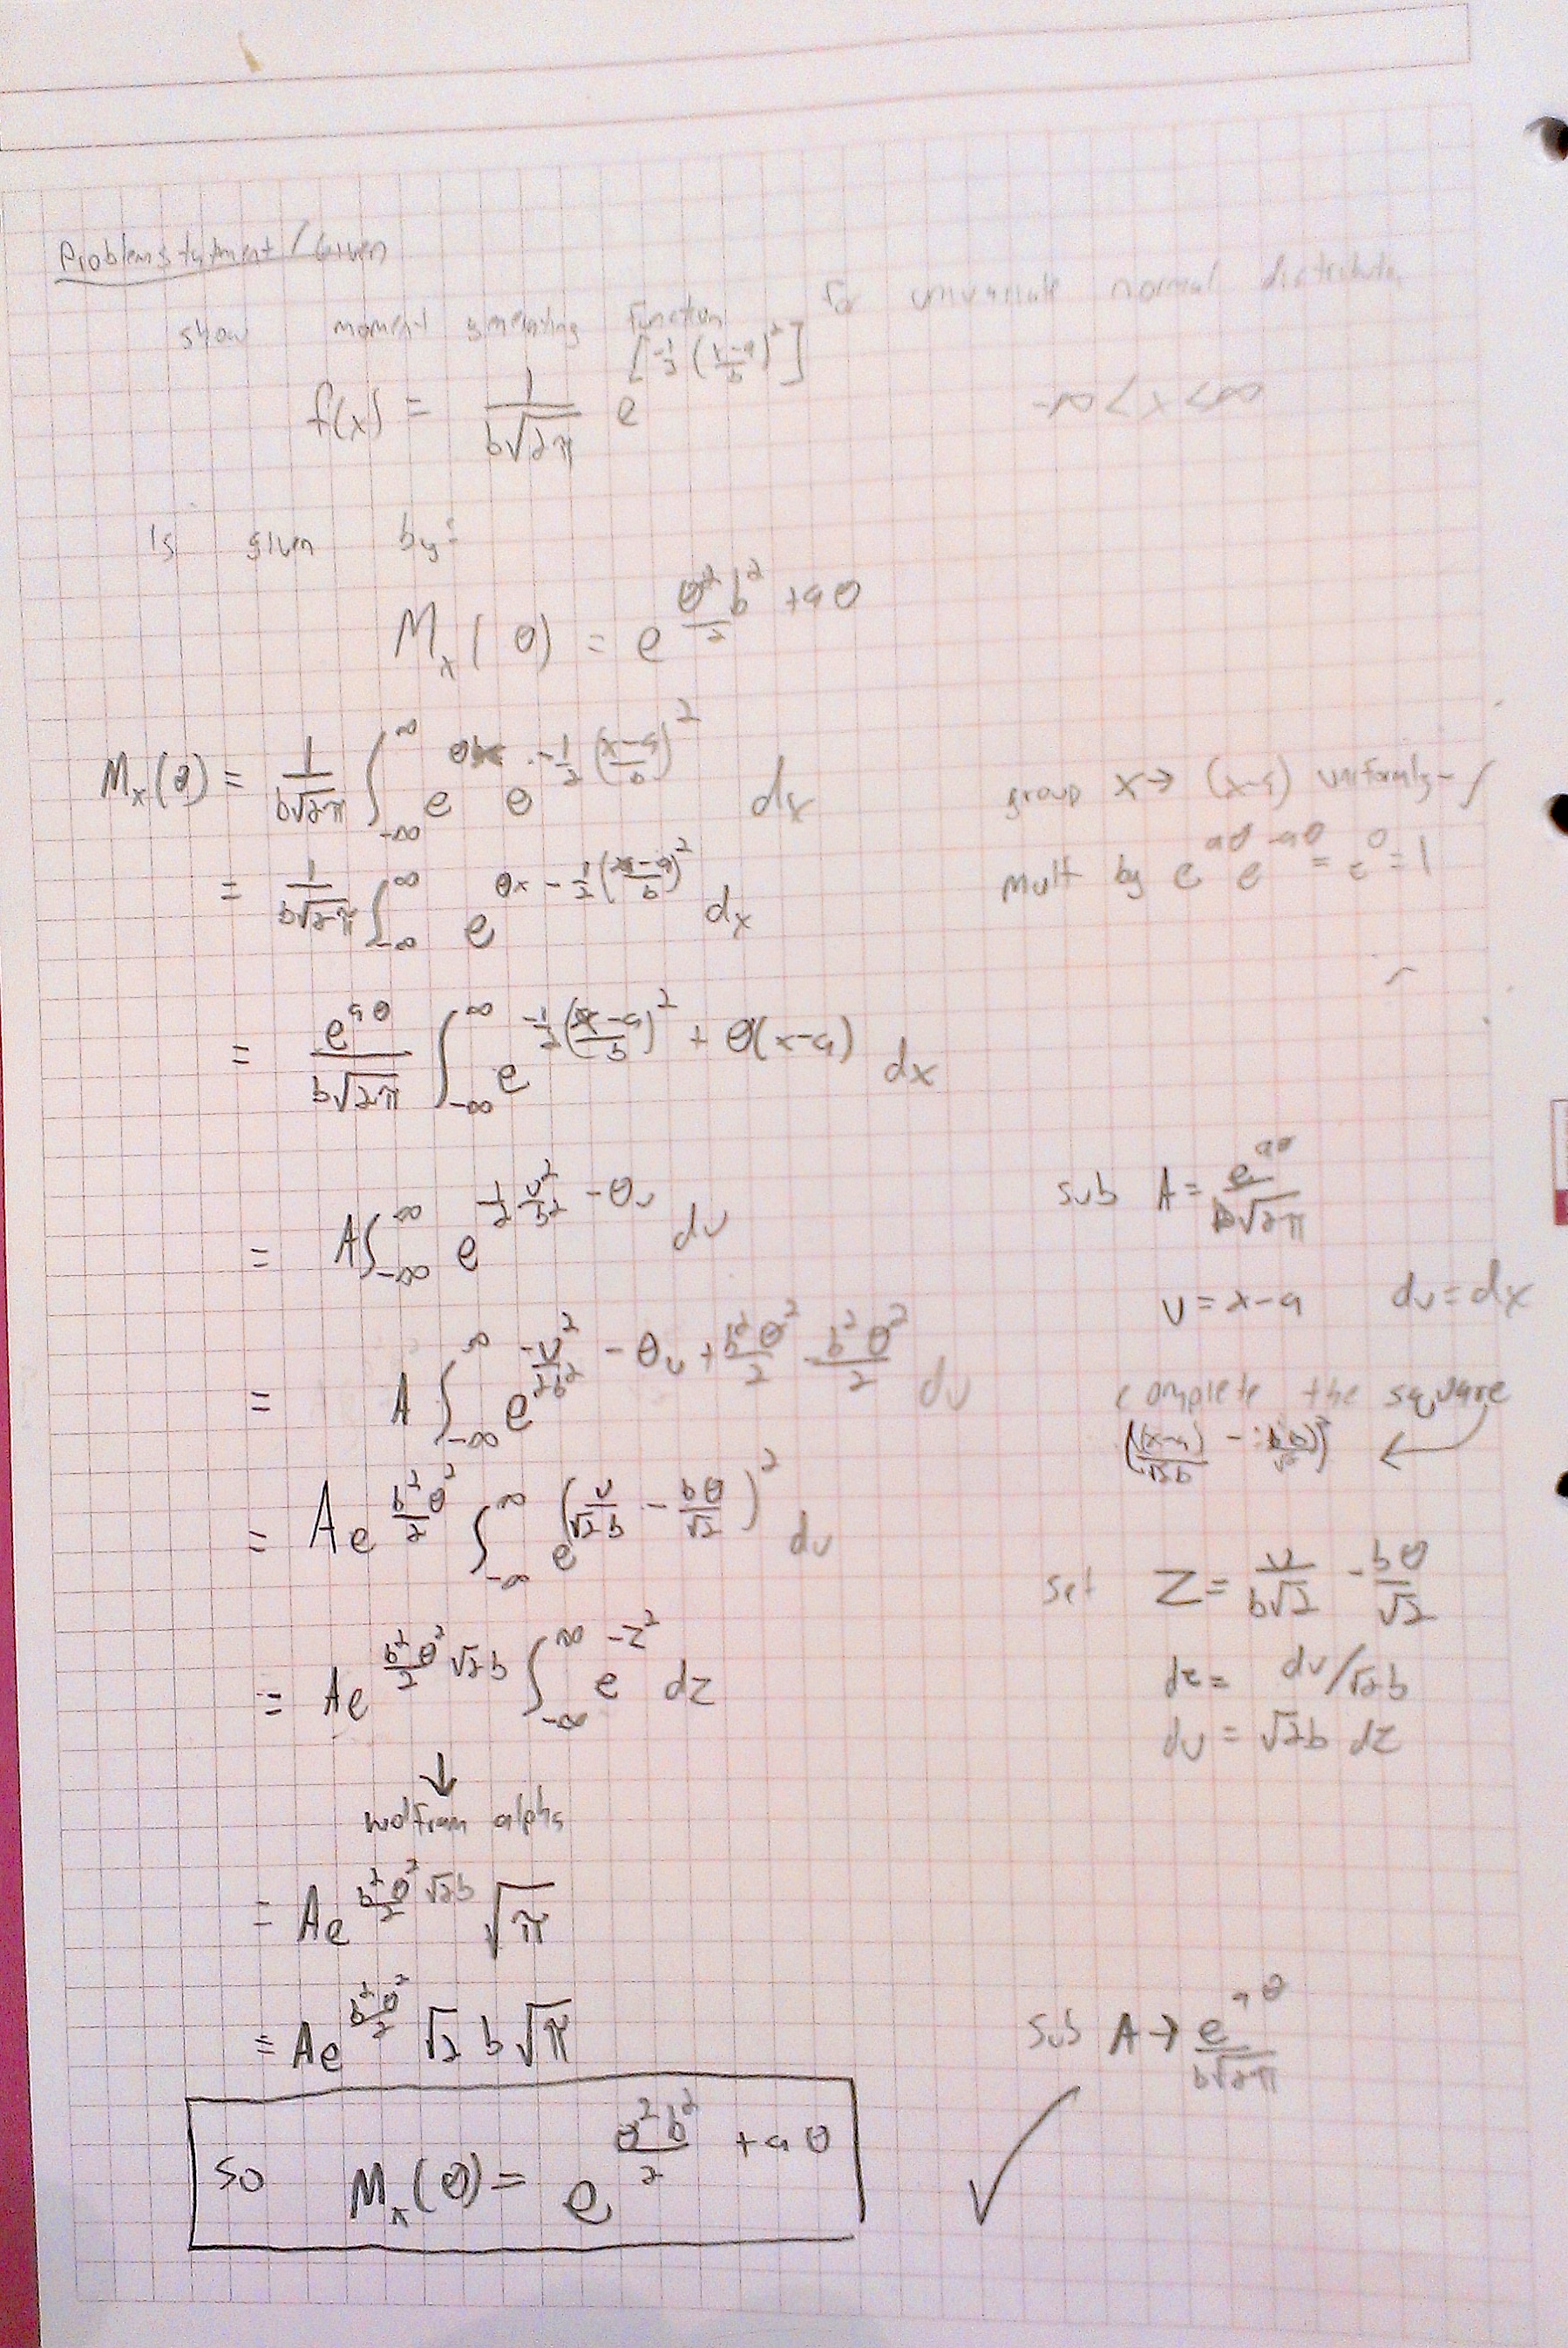
\includegraphics[scale=0.22]{Problem2.jpg}
\end{figure}




\vspace{3in}





%%%%%%%%%%%%%%%%%%%%%%  << 3 >>  %%%%%%%%%%%%%%%%%%%%%%%%
\section{Problem 3}
If {\bf x} and {\bf y} are independent random variables, show that:

\begin{equation}
	\sigma^2(xy) = \sigma^2(x)\sigma^2(y) + \lambda^2(x)\sigma^2(y) +  \lambda^2(y)\sigma^2(x)
\end{equation} 

\noindent Using the notation from {\bf Appendix A}.


\begin{displaymath}
	\sigma^2(xy) = E(xy - E(xy))^2
\end{displaymath} 

\begin{displaymath}
	\sigma^2(x) = \mu_{20}
\end{displaymath}

\begin{displaymath}
	\sigma^2(y) = \mu_{02}
\end{displaymath}

\begin{displaymath}
	\lambda(x) = \lambda_{10}
\end{displaymath}

\begin{displaymath}
	\lambda(y) = \lambda_{01}
\end{displaymath}

\noindent \newline \newline {\bf \Large Solution:}

\noindent	Using Appendix A and the given identities, I was able to prove the above equation. In addition to those given, I used the identity used for problem {\bf 1g}. I found it to be very helpful in the proof. 



\begin{figure}[hbtp]
	\noindent 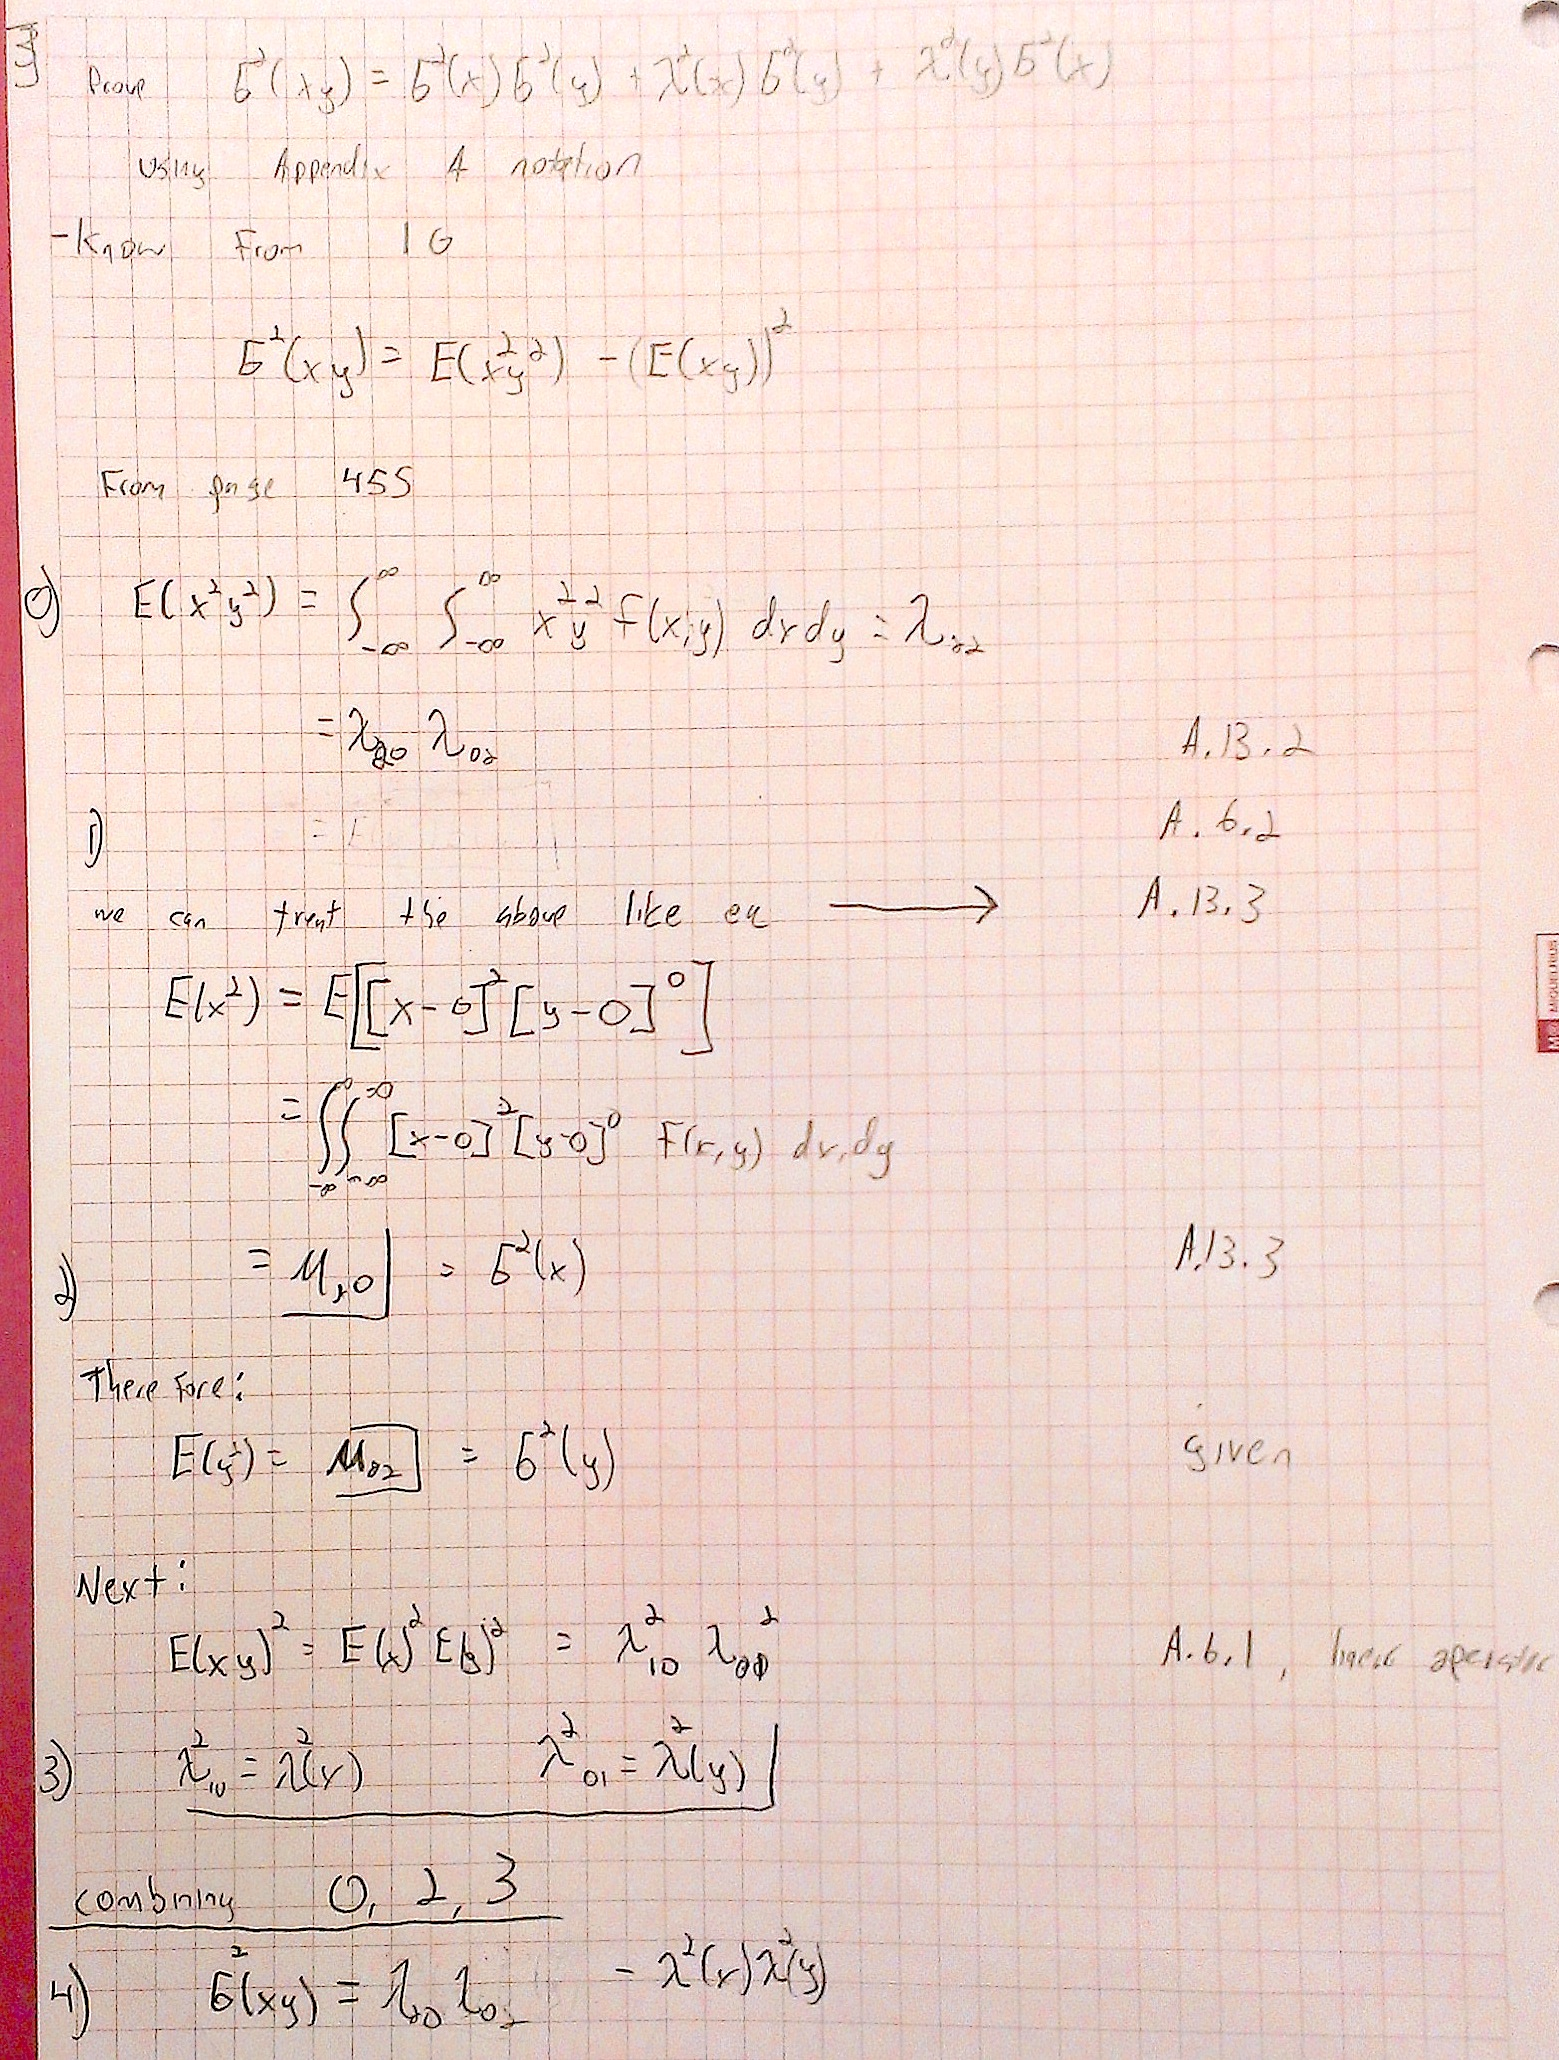
\includegraphics[scale=0.29]{Problem3Page1.jpg}
\end{figure}


\begin{figure}[hbtp]
	\noindent 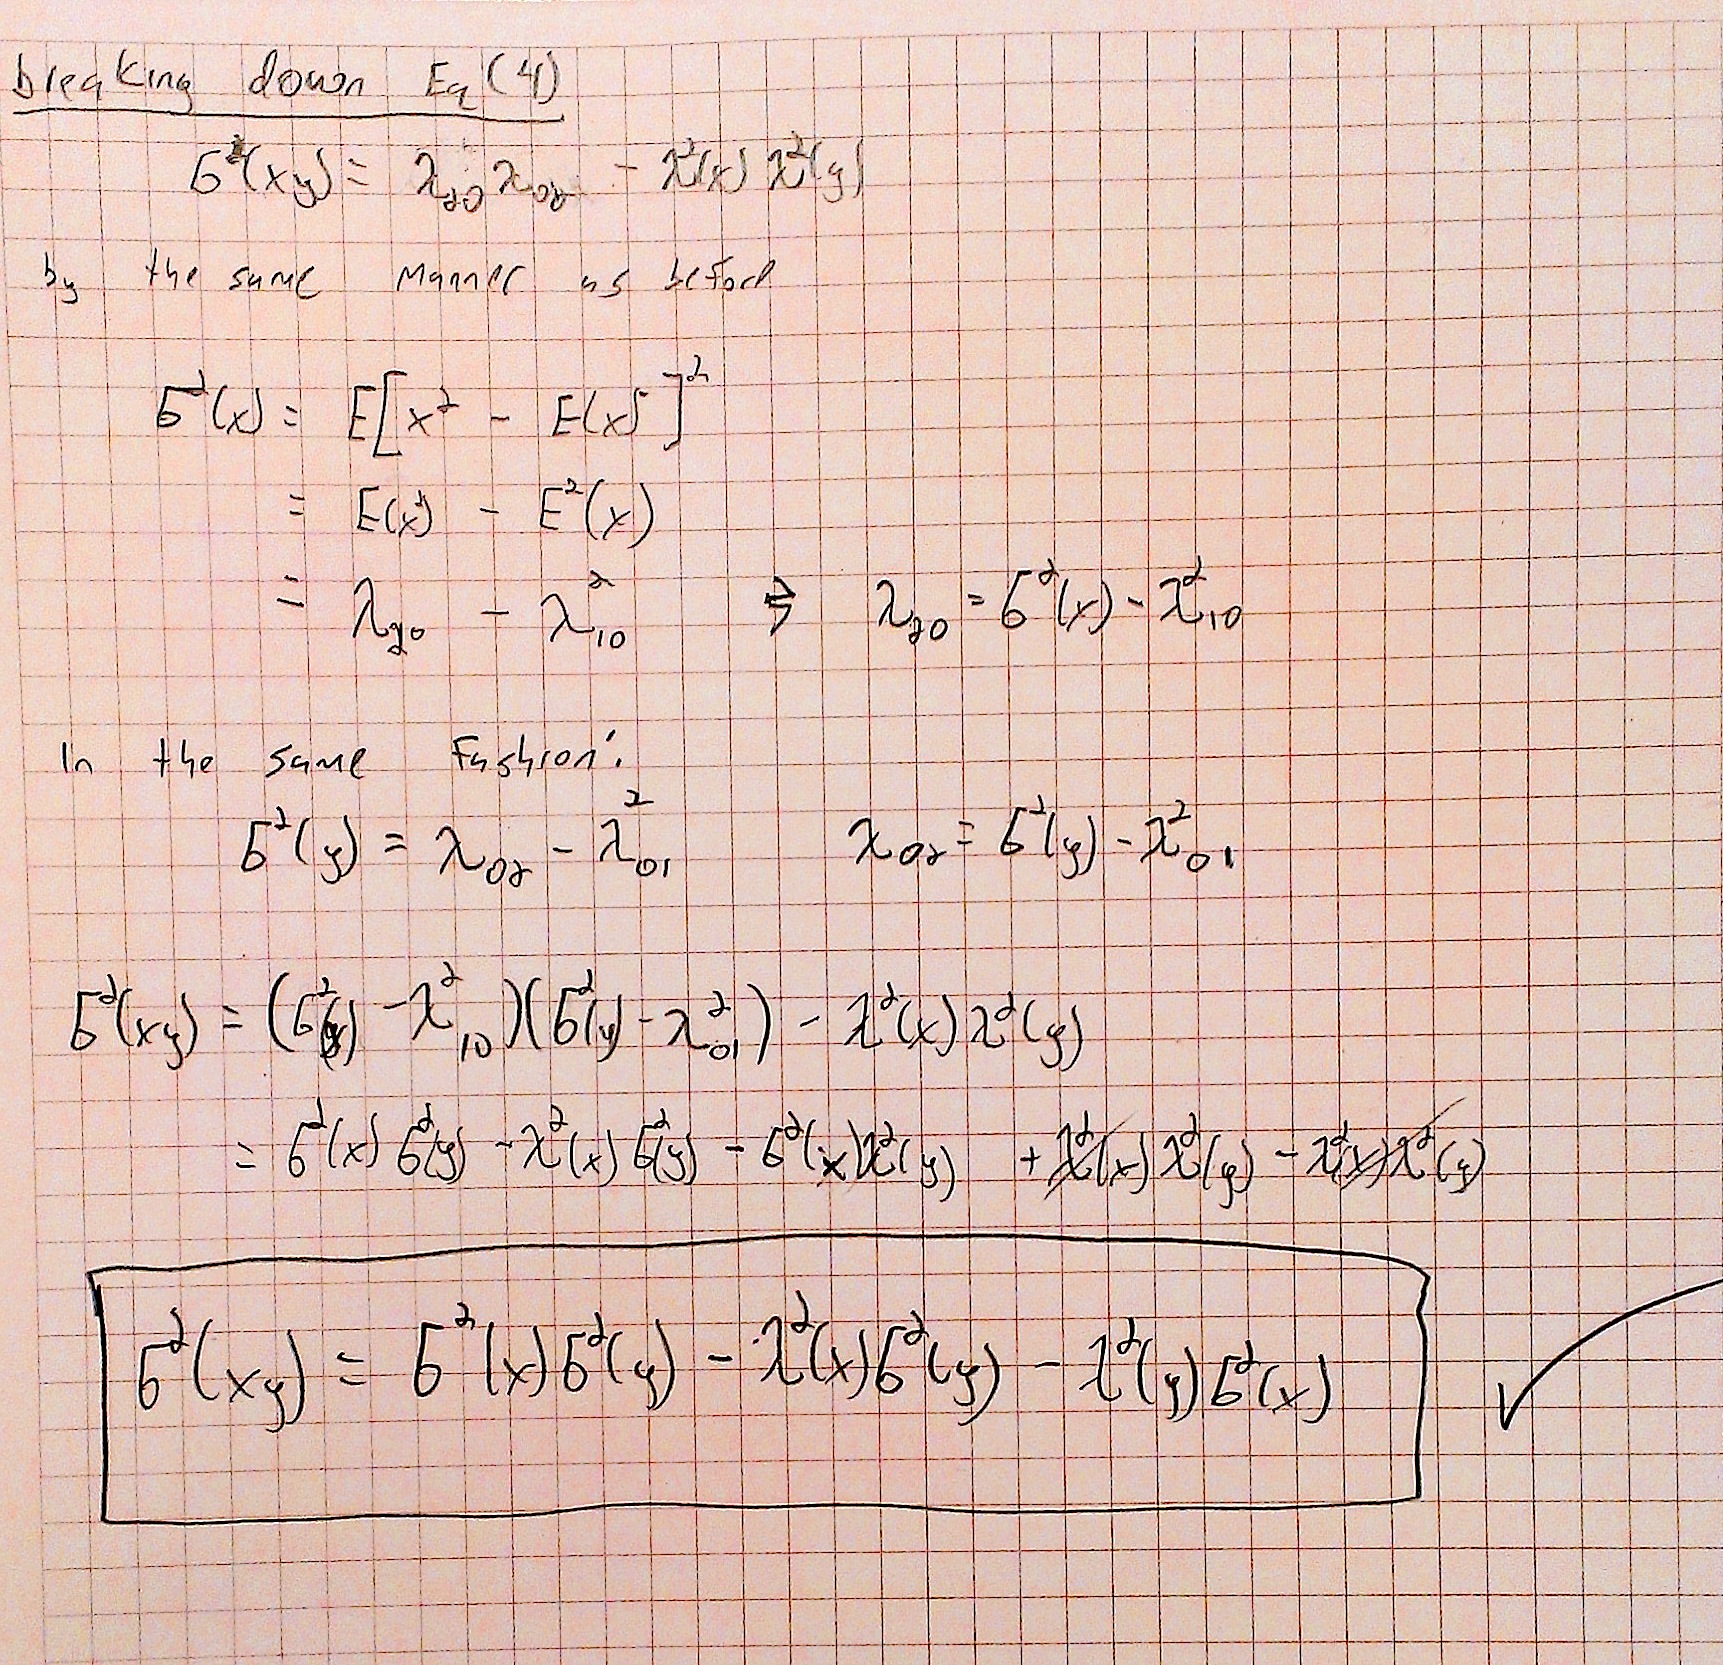
\includegraphics[scale=0.25]{Problem3Page2.jpg}
\end{figure}

\vspace{8in}

%%%%%%%%%%%%%%%%%%%%%%  << Appendix >>  %%%%%%%%%%%%%%%%%%%%%%%%
\section{Appendix A}
The MATLAB code for this assignment is pretty brief, and has been seen throughout this paper. The entirety of the code used is shown here. 

\begin{lstlisting}
	clc;clear all;close all; format compact
	% Go back and comment the shit out of this!!!
	
	%% 1
	% 1a
	syms x y k
	
	k = 1/int(int((x^2+y^2),0,2),1,3);
	k = eval(k);
	disp(['k is:  ',num2str(k)]);
	
	% 1b
	clear x; clear y; 
	fun     = @(x,y) k*( x.^2 + y.^2);
	ymin    = 2;
	ymax    = 3;
	xmin    = 1; % maybe 0
	xmax    = 2;
	P_1B    = quad2d(fun,xmin,xmax,ymin,ymax);
	% P =int(int(k*(x^2 + y^2),2,3),1,2);
	disp(['Probability 1B:  ',num2str(P_1B.*100),'%']);
	
	% 1C
	
	% P =int(int(k*(x^2 + y^2),1,3),1,2);
	P_1C    = quad2d(fun,1,3,1,2);
	disp(['Probability 1B:  ',num2str(P_1C.*100),'%']);
	
	% 1D
	fun     = @(x,y) k*( x.^2 + y.^2);
	ymin    = @(x) 4-x;
	ymax    = 3;
	xmin    = 1; 
	xmax    = 2;
	
	P_1D    = quad2d(fun,xmin,xmax,ymin,ymax);
	disp(['Probability 1D:  ',num2str(P_1D.*100),'%']);
	
	% 1E
	xmin    = 0;
	xmax    = 1;
	ymin    = @(x) 4-x;
	ymax    = @(x) 4-x;
	P_1E    = quad2d(fun,xmin,xmax,ymin,ymax);
	disp(['Probability 1E:  ',num2str(P_1E.*100),'%     (0 expected, no volume)']);
	
	% 1F
	fun_x   = @(x) k*(x.^2 + (3)^2);
	Hy      = @(y) k*( 2*y.^2 + 8/3);
	xmin    = 0;    xmax    = 1;
	y_value = 3;
	P_1F    = quad(fun_x,xmin,xmax)/Hy(y_value);
	disp(['Probability 1F:  ',num2str(P_1F.*100),'%']);
	
	%1G -Standard Deviation
	% marginal distribution, how to do this in matlab cleanly?
	Gx      = @(x) (2*k*(3*x.^2 + 13))/3;
	E_x2    =  quad(@(x) (x.^2).*Gx(x),0,2);
	E_x_2   = (quad(@(x) x.*Gx(x),0,2))^2;
	
	disp(['E(x^2):  ',num2str(E_x2)]);
	disp(['E(x)^2:  ',num2str(E_x_2)]);
	Sigma_x = sqrt(E_x2 - E_x_2);
	disp(['sigma_x:  ',num2str(Sigma_x)]);
	
	
	% 1H
	P_1H    = quad2d(fun,1,2,1,2)./quad(Hy,1,2);
	disp(['Probability 1H:  ',num2str(P_1H.*100),'%']);
\end{lstlisting}

\end{document}














